\documentclass[11pt,a4paper]{article}
\usepackage[margin=2.1cm]{geometry}
\usepackage{amsmath,amssymb,booktabs,graphicx,hyperref}
\graphicspath{{docs/figures/}}
\hypersetup{colorlinks=true,linkcolor=blue,urlcolor=blue}
\title{Longer Lorenz PINN Trajectories and the Residual-Direction Hypothesis}
\author{Project research update}
\date{22 November 2026}
\begin{document}
\maketitle

\begin{abstract}
The project's prespecified 40-run test found no reliable predictive benefit
from a PINN residual's alignment with one locally expanding direction.
The original global Lorenz-63 PINNs were accurate only over windows of length
one. We trained eight consecutive hard-initial-condition PINNs over a
length-two window, passing each predicted endpoint to the next model without
using internal reference states. In a fixed 8-window by 5-seed evaluation,
35 of 40 trajectories remained within error one throughout the window;
all five failures were on one initial-condition window. The original
directional analysis repeated on these trajectories still found no
held-out gain from either the backward Lyapunov vector or the leading
finite-time singular vector. An oracle feature using the full tangent
propagator did add held-out information at longer horizons, including after
controls for elapsed time. This is a post-hoc research update, not a new
confirmatory result or a practical predictor.
\end{abstract}

\section{Question and context}
Turinici's time-weighting paper~\cite{turinici} studies \emph{when} to weight
PINN equation violations during training. Our submitted project
report~\cite{projectreport} also asked a separate question: does the
\emph{direction} of a trained PINN's ODE residual predict its future
trajectory error beyond residual magnitude? The original analysis used
Lorenz-63 and tested alignment with the backward Lyapunov vector $b_1$ and
the leading finite-time singular vector $s_1$. Its fixed decision rule was
not met by either direction. We sought a more accurate PINN before revisiting
that diagnostic question.

\section{Model and evaluation}
We call this a \emph{sequential time-domain decomposition PINN}, or a
\emph{time-marching PINN}. These are established terms for successive
time-segment networks~\cite{penwarden}. Our construction is related to
hard-constrained sequential PINNs~\cite{roy}, but the float32 endpoint
transfer is continuous only to about $10^{-6}$ and we do not enforce
derivative continuity; we do not claim exact reproduction of that method.
Each run trains eight consecutive networks on intervals of length $L=0.25$.
All use four 64-unit tanh layers. Within segment $k$, the network output is
\begin{equation}
\widehat{x}_k(\tau)=x_{k,0}+\frac{\tau}{L}
\bigl[g_k(\tau)-x_{k,0}\bigr],\qquad 0\leq\tau\leq L.
\end{equation}
This enforces the starting state exactly. The first $x_{k,0}$ is the supplied
initial condition; subsequent starting states are the \emph{preceding PINN's
predicted endpoints}. No interior reference states enter training. Each
network receives 4,000 Adam updates with 256 stratified collocation times
per update. We fixed this construction on pilot window 0, then ran windows
1--8 with seeds 0--4 without changing settings. A high-accuracy DOP853
reference is used only to evaluate error and calculate oracle tangent data.

On the pilot, a single hard-initial-condition PINN over $T=2$ had median
trajectory error 6.052, whereas the piecewise model had median error 0.0259
and maximum error 0.154. The training budgets and network counts differ;
the pilot compares complete setups rather than isolating segmentation.

\begin{table}[h]
\centering
\caption{Trajectory accuracy of the fixed piecewise PINN over $T=2$.}
\begin{tabular}{lr}
\toprule
Measure & Result\\
\midrule
Runs & 40 (8 windows $\times$ 5 seeds)\\
Median of per-run median errors & 0.0433\\
Median of per-run maximum errors & 0.1823\\
Runs below error 1 throughout & 35/40\\
Runs below error 1 for at least 90\% of the window & 35/40\\
\bottomrule
\end{tabular}
\end{table}

All five failures occur on window 1, with late maximum errors between about
3.05 and 8.21. Every run on windows 2--8 remains below error one throughout.
Figure~\ref{fig:validation} shows the full distribution.

\begin{figure}[t]
\centering
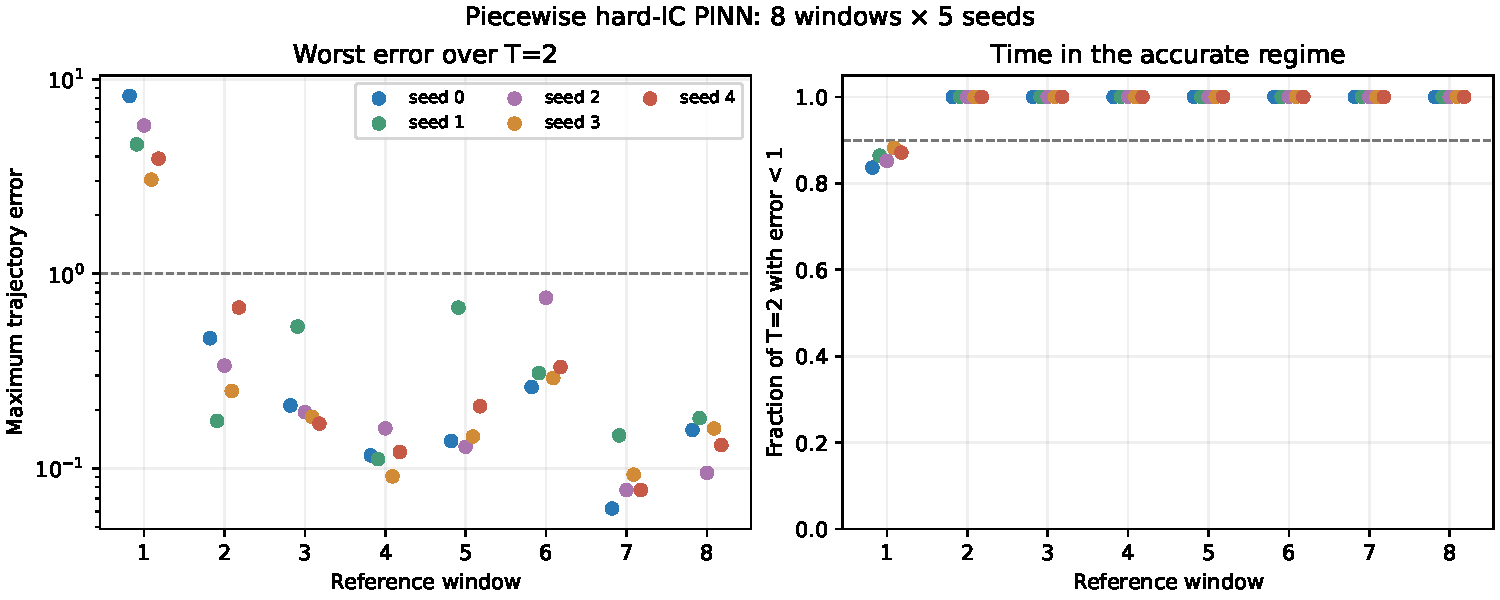
\includegraphics[width=0.98\linewidth]{piecewise_pinn_validation_40runs.pdf}
\caption{Accuracy of all 40 fixed-setting piecewise PINN runs. Each point is
one window/seed pair. Dashed lines mark maximum error one and 90\% of the
window below error one.}\label{fig:validation}
\end{figure}

\section{Residual direction and full amplification}
We reused the original leave-one-initial-condition-window-out analysis on
the 40 new trajectories. Exact segment joins were excluded from predictor
times because the piecewise derivative has different one-sided values there.
The baseline predictor used log residual norm. Adding either $b_1$ or $s_1$
alignment gave negligible or negative held-out $R^2$ gains at all five
horizons; neither passed any horizon of the original four-part rule.

\begin{table}[h]
\centering
\caption{Gain in held-out $R^2$ beyond pointwise residual magnitude.
The last column is an oracle using $\|\Phi(t+\Delta,t)r(t)\|$.}
\begin{tabular}{rrrr}
\toprule
Horizon $\Delta$ & $b_1$ alignment & $s_1$ alignment & Full amplification\\
\midrule
0.05 & $-0.0003$ & $-0.0041$ & $-0.0005$\\
0.10 & $-0.0001$ & $-0.0020$ & $+0.0027$\\
0.25 & $-0.0099$ & $+0.0029$ & $+0.0513$\\
0.50 & $-0.0176$ & $+0.0010$ & $+0.1948$\\
1.00 & $-0.0002$ & $-0.0013$ & $+0.3068$\\
\bottomrule
\end{tabular}
\end{table}

We tested whether the oracle gain merely reflects elapsed time by adding
$t$ and $t^2$ to the residual-size baseline. The full-amplification feature
still added held-out $R^2$ of $+0.046$, $+0.191$, and $+0.360$ at horizons
0.25, 0.5, and 1.0. After excluding the late-failing window 1, the gains
were $+0.026$, $+0.135$, and $+0.169$. A further oracle baseline with
current true error also left positive gains. The propagator and current true
error require the reference trajectory: these analyses probe mechanism, not
a deployable error indicator.

\section{Limits and next test}
This model was chosen after the original negative result, so its directional
analysis is exploratory even though settings were fixed for the 40-run
extension. Five seeds share each of only eight initial-condition windows.
The piecewise state joins to approximately $10^{-6}$ in the pilot, but slope
jumps reach 4; the original smooth-trajectory Duhamel quadrature has not
been corrected at those joins and is not interpreted here. Window 1 fails
late for every seed. Bootstrap intervals based on runs are descriptive and
do not constitute 40 independent initial-condition replications.

The next decisive study should freeze this model and analysis before using
new Lorenz initial-condition windows. It should estimate uncertainty at the
window level, correct Duhamel quadrature across joins, and test a causal
history integral of residuals against simple time and trailing-history
controls. The current evidence supports a concrete model improvement and
the continued absence of a one-vector diagnostic, while leaving a practical
predictor and generality to new systems open.

\begin{thebibliography}{9}
\bibitem{turinici} G. Turinici, \emph{Regime-Aware Time Weighting for
Physics-Informed Neural Networks}, arXiv:2407.21642v2, 2024.
\bibitem{projectreport} \emph{Project Report -- Differential Equations -- 2},
submitted project report, available in this repository under \texttt{docs/}.
\bibitem{penwarden} M. Penwarden, A. D. Jagtap, S. Zhe, G. E. Karniadakis,
and R. M. Kirby, \emph{A unified scalable framework for causal sweeping
strategies for physics-informed neural networks and their temporal
decompositions}, Journal of Computational Physics 493 (2023), 112464.
\bibitem{roy} P. Roy and S. Castonguay, \emph{Exact Enforcement of Temporal
Continuity in Sequential Physics-Informed Neural Networks},
arXiv:2403.03223v2 (2024).
\end{thebibliography}
\end{document}
